\documentclass[pdfpagelabels=false,plainpages=true]{acm_proc_article-sp}

\usepackage{color}
\usepackage{hyperref}

\begin{document}

\title{Course-specific search engines: Semi-automated methods for identifying
  high quality topic-specific corpora} 

\numberofauthors{2}
\author{
  \alignauthor
  Neel Guha \\
  \email{neelguha@gmail.com}
  \alignauthor
  Matt Wytock \\
  Google, USA
  \email{mwytock@google.com}
}

\maketitle
\begin{abstract}
Web search is an important research tool for many high school courses. However,
generic keyword search engines have a number of problems that arise out of
not understanding the context of search (the high school course),
leading to results that are off-topic or inappropriate as reference material. In
this paper, we introduce the concept of a course-specific search 
engine and build such a search engine for the Advanced Placement course on US
History; the results of which are evaluated by subject matter experts (high
school teachers) and judged to be overwhelmingly superior to existing search engines. We
then develop two algorithms for identifying high quality documents: one 
based on textual similarity to an authoritative source and another using structured
data from knowledge bases. Initial experimental results indicate that
these algorithms can be used to automate the creation of course-specific search
engines with minimal manual supervision.
\end{abstract}

\section{Introduction}

Over the last decade, the World Wide Web has become one of the primary sources
of information for students. This is especially the case for high school
subjects such as history, which often have projects that require the student to 
perform independent research. Unfortunately, students encounter difficulties
with mainstream keyword-based search engines (such as Bing or Google); 
consider two examples of queries that might arise in the context of a course
on US History: the query [boston tea party] brings up the home page for the
Boston chapter for the political organization called the ``Tea Party'' and the
query [benjamin franklin] brings up pages about Benjamin Franklin
Plumbing. These queries also bring up pages that are targeted at elementary
school students and user-generated content such as Yahoo Answers, which are not
considered good reference material by most teachers.

Traditional methods in information retrieval rely on term-based scoring between
the query and the document via the vector space model \cite{salton1975vector} or
more sophisticated Ngram models to ensure on-topic results. However, for many
reasonable queries in the academic research context, such methods are
fundamentally limited. We group problems that arise into three categories:

{\bf Off-topic results}. Often, many of the results are off-topic in the
research context. For example, [benjamin franklin] brings up results about a
plumbing service with that name and [gold rush] brings up pages related to Gold
Country tourism. The problem is especially severe with queries involving
names of places, which bring up results about restaurants, real estate
offerings, and other local services. Since students are learning the topic by
conducting exploratory searches, they cannot be expected to frame the best query
which exacerbates the problem. 

{\bf Inappropriate sources}. Web search results often include a number of sources
that do not meet the standard for research material in an academic course. Some
egregious examples include user-generated content (such as forums and Yahoo answers), 
sites offering essays from other students, and biased sites (such as
ConfederateAmericanPride.com). Unfortunately, these results are interspersed
with those from reputable sites leaving the student to sift through result
set. Unlike off-topic results which are mostly just a nuisance, these results
often lead the student astray.   

{\bf Wrong level}. Even search results that are on-topic from reputable
a site may be targeted at the wrong level. For example, [thomas jefferson]
returns a page from the children's version of the Library of Congress
website while  more detailed queries often return papers from graduate level
work. Typically web pages are not explicitly labeled with the level of
the intended audience making it difficult to formulate an query that returns
appropriate results.

In practice, the user must compensate for these search engine deficiencies by
constructing more specific queries. Unfortunately, this both requires an
intimate knowledge of the subject, which by definition the student does not yet
have, and often eliminates potentially good results. The root of the problem is
that a two or three word query does not communicate the context in which the
student is trying to use the search engine. Thus, the general purpose
search engine must have appropriate results for all users and cannot
provide the best possible results for a particular student in a specific
educational context. 

Our solution is to construct a specialized search engine for every academic
course. We use a popular high school course, AP US History (APUSH)---taken by
over 400,000 students in 2011 \cite{wikipedia}, as 
our target educational context and show how we can construct a search engine
that captures the 
richness of the web while avoiding some of the problems associated with generic
search engines. In order to run the search engine, we use the Google Custom
search engine platform  (\url{http://google.com/cse}) which allows us to
restrict the corpus of our search engine to a set of url patterns or sites. The
CSE platform takes care of the cumbersome tasks of crawling the web, building an
index and running the search engine. This has allowed us to not only build a
search engine for APUSH, but to also make it widely available to students taking
the course.     

We first demonstrate the utility of this course-specific search engine by creating
a reference search engine with a manually curated set of sites. In a
blind side-by-side evaluation by domain experts (APUSH teachers), this search
engine is overwhelmingly preferred to Google. However, manually curating
thousands of sites is a time-consuiming process and thus we develop two
automated algorithms. In order to do so, we make the assumption there exists a
textbook, or other authoritative source, which describes the course content.
We propose two algorithms that utilize this source: one using textual similarity and
another using structured data from knowledge bases. Our experimental results
indicate that these algorithms significantly reduce the amount of manual work
required to create a course-specific search engine.

\subsection{Related work}

There has been substantial work in the area of topic-specific ranking focused
around exploiting the link structure of the web to identify clusters of
documents that are on the same topic. For example, this structure can be
exploited to create a topic-specific Page Rank for influencing ranking
\cite{haveliwala2003topic, hsu2006topic} or to influence the order in which
pages should be crawled \cite{buntine2004scalable}. In contrast, our work uses the
text content of an authoritative source (the course textbook) to define
topic-specific ranking algorithms.

Focusing on the domain of search engines for the educational context, the most
closely related systems are those of PubMed, Web of Science and Google
Scholar, which search specialized corpora of scientific research
\cite{jacso2005google}. Unlike these systems which include only
peer-reviewed scientific articles, our course-specific search engines
endeavor to include all of the useful educational material that can be found on
the web. 

We are aware of very little work on the use of knowledge bases to influence the
results shown in search. Some exceptions are \cite{jiang2009learning}, which explores
using ontologies for characterizing the user and \cite{guha2003semantic} which
show how search results can be augmented with snippets from a knowledge base.   

\section{Reference search engine}

In order to evaluate the relative performance of a search engine for the AP US
History course, we first create a reference search engine based on a standard textbook
\cite{textbook}, which is available in PDF form. As described above,
we use the Google CSE platform which allows us to specify the corpus for our a
search engine as a set of url patterns.

If we knew all the queries that students will issue in the APUSH context, a
brute force approach would be to go through the search results returned by
Google and manually pick the good results. Clearly, this is not possible both
because the queries are not known apriori and because of the magnitude of manual
work that would be required. We therefore approximate this by computing likely
queries from the textbook and then, by doing the curation at the site level as
opposed to the page level. This curated set of sites will then form the corpus
of our reference search engine.

Most history related queries include one or more proper nouns (people, events,
places, etc.). Thus, we use the digital version of the textbook \cite{textbook}
to extract all the proper nouns, using simple syntactic cues such as
capitalization and punctuation. This method identifies 1206 distinct proper
nouns, occurring a total of 11241 times in the text. We then form queries out of
tuples of proximately occurring proper nouns and retrieve the top ten results
from Google. The 132,145 results for these queries come from 23393 sites. There are
1757 sites which appear in at least 10 results and these account for 70.2\% of
all results. We manually examined each of these sites to put them into two
buckets: those that were bad (either off-topic (e.g., trulia.com, yelp.com)
or not appropriate for academic work (e.g., answers.yahoo.com, wikianswers.com))
and those that were good. 768 were off-topic or not appropriate, leaving us with
989 good sites. So, if we were to randomly select sites, only 56\% of the
selected sites will be good. 

\begin{figure}
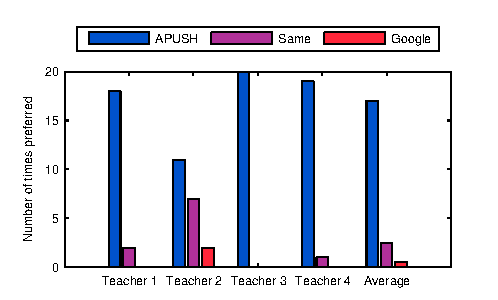
\includegraphics{teacher_eval}
\caption{Side-by-side comparison of the APUSH search engine and Google}
\label{fig-eval}
\end{figure}

We created a custom search engine using the good sites (available at
\url{http://guha.com/apushcse.html}). In order to evaluate this search engine,
we collected a set of 20 queries (included in Appendix \ref{app-queries}) and
asked a set of 4 history teachers to compare results from Google versus results
from the custom search in a blind side-by-side test setup. They were asked to
assign one of the following ratings to each side-by-side: side A/B is better,
side A/B are about the same. As can be seen in Figure \ref{fig-eval}, the
course-specific custom search engine is substantially preferred.

\section{Methods for automation}

Our long term goal is to be able to create a course-specific search engine from
the course textbook with minimal manual supervision. The reference search engine
described above involved manual curation of thousands of sites, a process that
is very time-consuming and expensive. Our goal is to automatically distinguish
between sites that produce off-topic results / sites that are inappropriate for
academic usage and sites that may be used for academic work.  Rather than
attempting a binary classification of sites into ``good'' and ``bad'', we rank sites
based on the likelihood of them returning good results for APUSH searches. A CSE
can then be configured to include just the top N sites or better, or to prefer
sites that are ranked higher. 

\textcolor{red}{Links should be made here about topic-specific
  PageRank. Essentially this is a course-specific quality score.}

The root of the problem is that a two or three word query does nt communicate
the context in which the student is trying to use the search engine, i.e., the
APUSH course.  When an off-topic site, such as Benjamin Franklin Plumbing, comes
up for a history query, such as [benjamin franklin], the problem is that the
query is inherently ambiguous and there is no way to communicate the context of
the search (i.e., the APUSH course) to the search engine.  Our overall approach
is to use this larger context in an offline process to construct the right
collection of sites. 

We now describe a progression of algorithms that can be combined to improve on
this baseline. We start with a classical information retrieval style analysis of
the content of search results page and of the APUSH textbook. Sites that are
more similar to the APUSH textbook are more likely to yield better search
results. In the next step, we use a knowledge base of facts about the real world
entities to improve the ranking obtained by just textual similarity. Finally, we
present a relevance feedback based learning algorithm that improves the search
engine based on user interaction with search results. 

\subsection{Authoritative documents}

\textcolor{red}{Instead of writing this section in terms of an explanation of
  TF-IDF and vector space models which are classic methods, I would rephrase this
  as an alternative way to compute a topic-specific quality score using an
  authoritative reference which is a new idea.}

\textcolor{blue}{I tried to, but I couldn't come up with a satisfactory way of
  saying this. Could you please help me?} 

Classical information retrieval is based on the notion of similarity between two
pieces of text, typically, the query and the web page.  In our case, we compute
the similarity between the pages on a site and the APUSH textbook. Sites that
are more similar to the APUSH textbook should  be more likely to return better
results. 

One of the most commonly used similarity measures is the cosine similarity
metric based on the vector space model of documents \cite{salton1975vector}. In
this model, each document is a vector in an N dimensional where each term in the
corpus is a dimension. The coordinates of a document along the ith axis is given by by a
product of the term's frequency in the document (TF) and the a measure of how
significant that term is in the corpus. The later is usually measured by Inverse
Document Frequency (IDF), which is the log of the inverse of the number of
documents in the corpus that the term appears in. The similarity between two
documents in this model is the cosine of the angle between the vectors between
the two documents. 

Aiand Bi are the tf-idf for each term i in the corpus, for the two documents. We
compute the similarity of a site to the APUSH textbook as follows. We retrieved
the content of 110,121 of the 132,145 pages returned by Google as results for
the queries that we used to create the reference search engine (many pages could
not be retrieved either because the sites blocked our robot or because the site
was down). After stripping the pages of all the HTML markup and javascript, we
stem the words on each page (using the Porter Stemmer
\cite{porter1980algorithm}) and extract the terms from (the pages from) each
site along with their frequency of occurrence. We also stem all the terms in the
APUSH textbook. We then compute a similarity score between each site and the
APUSH textbook using the cosine similarity metric.

While textual similarity based metrics are very powerful for identifying
off-topic sites, they are not capable of identifying sites that are on-topic,
but likely inappropriate for academic purposes (such as answers.yahoo.com or
ConfederateAmericanPride.com). These sites are indeed on-topic, but pure
similarity based metrics cannot detect the bias. For this, we need some form of
human judgement. We next describe a mechanism for getting this by analyzing the
search engine's usage. 

\subsection{Knowledge based approach}

Most queries and web documents are about real world entities.  This realization
has led many of the big search engines to build various kinds of knowledge
bases to augment their search results \textcolor{red}{Nice to cite blog post
  here}. There has also been a lot of work in the area of the semantic web
and linked data \cite{berners2001semantic,bizer2008linked} which aim to build a
large distributed network of information about entities and the relations
between them. In this section, we describe how this source of information can be
used to improve the ranking based on simple textual similarity.  

Some types of entities lead to more off-topic results than others. For example,
places (e.g., Virginia, Maryland) are more likely to lead to results that are
not about history compared to US presidents since the former will bring up real
estate and local results. US Presidents in turn are more likely to bring up
off-topic results compared to Confederate Generals, since the former are more
likely to have institutions and places named after them. This relative preference
(Confederate Generals better than US Presidents better than Places) captures
some of the APUSH context. 

Our goal is to automatically identify the types that are more likely to give
good results and give greater preference to the sites that are pulled up for
queries that contain references to these kinds of entities. Before we can do
that, we need to map the proper nouns we extract from the text to entities and
the entities to types of entities. Ideally, we would like to do this in a
fashion that is not specific to history, but will work with little or no change
to many other subjects. To do this, we need a broad knowledge base about a large
number of entities, along with information about the type of each
entity. Wikipedia contains this kind of information about a large number of
entities and DBPedia makes this information available as a structured knowledge
base. Each ``thing'' in Wikipedia corresponds to an entity in DBPedia
(www.dbpedia.org) and each ``category'' in Wikipedia corresponds to a DBPedia
type. We will use DBPedia as the primary source of entities, types and for
mapping proper nouns to entities and entities to types. 

There could be many different proper nouns corresponding to a single real world
entity. For example, President Lincoln, Abraham Lincoln, Abe Lincoln, etc. all
refer to the same person. Similarly, a given proper noun (e.g., Washington) could
map to multiple different entities. We found that the most robust way of mapping
from proper nouns to candidate entities is to use search itself. For every
proper noun P, we issue the query [P site:wikipedia.org]. Each of the search
urls has the form http://en.wikipedia.org/wiki/<entity-id>. The first three entities
for each query are used as candidate entities for the corresponding proper
noun. Each entity may have a number of categories associated with it. For
example, the entity whose unique identifier is Abraham\_Lincoln has 29
different categories associated with it: American\_Presidents,
Illinois\_Lawyers, Assasinated\_HeadsOfState, etc. This mapping is done using
the RDF dumps from DBPedia. 

The next step is to assign a score to each category. The score is a measure of
the likelihood of a query containing a proper term that refers to an entity in
that category bringing up a site with on-topic results. The intuition behind the
scoring algorithm is as follows. A course, such as APUSH, is about certain
categories of entities and the relationships between them. These categories
should be assigned higher scores. An example of such a category would be
American\_Presidents. There will be a number of other categories that also
appear, but only incidentally. These should get lower scores. Examples of such
categories would be Illinois\_Lawyers and Noble\_titles. We would expect that a
larger fraction of the entities in a category that the course is about will
occur in the textbook compared to categories that appear incidentally. The score
for the $i$th category is given by
\begin{equation}
CategoryScore_i = \frac{\#Textbook_i}{\#DBpedia_i}
\end{equation}
where $\#Textbook_i$ and $\#DBpedia_i$ count occurences of entities in the
textbook and DBPedia, respectively. 

For example, the textbook contains references to 33 entities in the category
American\_Presidents, which, in DBPedia is associated with 44 entities, giving
this category a score of 0.75. On the other hand, even though the text contains
references to more Harvard\_University\_Alumni (34), a total of 6533 entities in
DBPedia are associated with this category, giving Harvard\_University\_Alumni a
much lower score than American\_Presidents. 

\begin{table}
\begin{center}
\begin{tabular}{|l|} \hline
19th-century presidents of the United States \\
United States Presidential Candidates \\
Oneida New York \\
Presidents of the United States \\
Whig Party \\
Presidency of James Monroe \\
Christian denominational families \\
\hline \end{tabular}
\caption{DBPedia categories for APUSH}
\label{tab-categories}
\end{center}
\end{table}

\begin{table}
\begin{center}
\begin{tabular}{|l|} \hline
Andrew Jackson \\
Martin Van Buren \\
Thomas Jefferson \\
James Monroe \\
Abraham Lincoln \\
James Buchanana \\
Zachary Taylor \\
William Henry Harrison \\
Russia \\
\hline\end{tabular}
\caption{DBPedia entities for APUSH}
\label{tab-entities}
\end{center}
\end{table}

Table \ref{tab-categories} gives some of the the categories that are considered
most relevant to APUSH. As can be seen, of the hundreds of thousands of categories in
DBPedia (which includes categories for rock stars, planets, etc.), the
ones that come up are indeed very apropos to US History.           
We then score each entity by summing the scores for the categories that it is
associated with. For example, the entity Abraham\_Lincoln gets a contribution
from each of the 29 categories that it is a part of. Table \ref{tab-entities}
gives some of the top-rated entities. 

\begin{table}
\begin{center}
\begin{tabular}{|l|} \hline
Whigs in Congress \\
President Harrison \\
President Monroe \\
James Monroe \\
President Johnson \\
Thomas Jefferson \\
President Adams \\
Second Bank \\
Andrew Jackson \\
President Van Buren \\
\hline\end{tabular}
\caption{Highest scoring proper terms for APUSH}
\label{tab-terms}
\end{center}
\end{table}

Next, we score each proper term by adding the scores of all the entities that it
could refer to. So, since ``Abraham Lincoln'' could refer to the president or the
movie with that name, each entity contributes a score. Table \ref{tab-terms}
gives some of the top-rated proper terms. Again, as can be seen, of the millions
of entries in DBPedia, the ones chosen are indeed very highly apropos to the
APUSH context.  

We then score each query based on the proper terms in the query. Finally we
score each of the sites based on the scores associated with the queries for
which they produced results. The score for the site is the average of the query
scores. This gives us a ranking of sites by the likelihood of them being a good
candidate for inclusion into the APUSH search engine. 

This approach reduces the probability of off-topic results occuring
for our query. By utilizing a topicality based scoring approach, it
eliminates results for non-APUSH interpretations of a
particular query.


\textcolor{blue}{Does the paragraph above communicate this?}

\textcolor{red}{We should tie this approach (and the topicality scoring
  approach) directly to the the 3 problems laid out in the introduction:
  off-topic, inappropriate, wrong level. In particular, 
  its clear that both deal with off-topic results easily but not so clear how
  they work for inappropriate and wrong level.}

\subsection{Relevance feedback}

Using relevance feedback to improve the performance of systems is an established
technique \cite{salton1997improving}. As the search engine gets used, we can
interpret clicks from the user as feedback. For example, if users repeatedly
skip results from a certain site (even when pages from that site are ranked
higher), preferring results from certain other sites, they are expressing a
judgement about the appropriateness of that site for APUSH. 

\textcolor{red}{First, describe how we use the labeled data to generate fake
  relevance feedback. It would be best to use the equation environment to make
  it easy to parse. }

\textcolor{blue}{Isn't this described below?}

Evaluating relevance feedback algorithms requires large amounts of usage
data, which we don't have. So, we instead reused some of the manually curated
sites to evaluate the utility of relevance feedback in our context. Of the sites
that had been manually curated, we randomly selected 50 good sites and 50 bad
sites. In practice, this list of good and bad sites would be obtained from usage
logs. We aggregate the good sites and bad sites, each, into a single composite
document, so that we have 2 large documents, one corresponding to the good sites
(GD) and another corresponding to the bad sites (BD). Then, for each site we are
trying to score, we compute the similarity of the site to GD and BD. The net
relevance feedback score is the Good Score minus the Bad Score. 

\textcolor{red}{Now, with the fake feedback data out of the way we can describe
  the two methods in a way that is agnostic as to whether the data is fake
  agnostic as to whether its real or fake data}. 

The overall score for the site is the score for similarity to the APUSH textbook + the score
for similarity to the good sites - score for similarity to the bad sites. 

We can also incorporate relevance feedback to incrementally improve
performance. As with relevance feedback for similarity scoring, we sample 50
good and bad sites from the manually curated list to simulate data from actual
usage of the search engine. We compute a relevance feedback score for each
category as follows. We take the categories associated with each query (from the
previous step) and propagate them to the sites associated with the query to get
a set of categories associated with each site. The score associated with each
category is (Ng-Nb)where Ngis the number of good sites associated with the
category and Nbis the number of bad sites associated with the category. Then, as
before, we propagate the category scores to the sites.  

\section{Experimental results}

\begin{figure*}
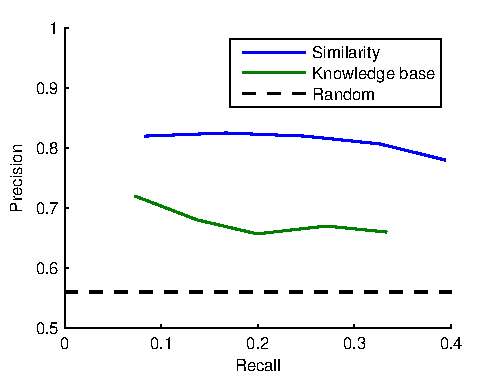
\includegraphics[width=3.45in]{expt}
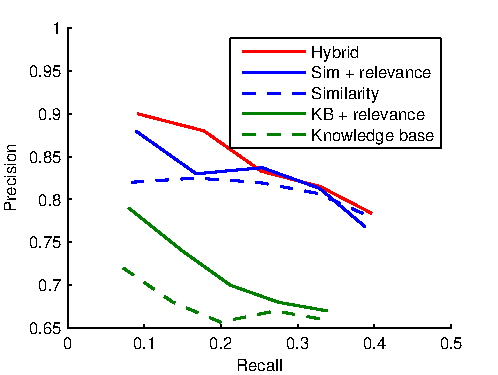
\includegraphics[width=3.45in]{expt_relevance}
\caption{Comparison of algorithms}
\label{fig-expt}
\end{figure*}

Of the 1453 sites we examined as part of the manual curation, 582 were good, 871
tended to give off-topic or inappropriate (i.e., bad) results. So, randomly
picking sites for inclusion into the search engine will lead to 40.05\% of the
sites being good. This forms the baseline for evaluating algorithms for
automating the curation. 

Each of our algorithms produces a list of sites ranked according to their
likelihood of producing good results for APUSH queries. We use the manually
curated list of good sites to measure how well an algorithm performs. The ideal
algorithm would rank each of the 989 good sites above the bad sites. Therefore,
a good metric for evaluating an algorithm is the number of good sites included
in the top 100, 200, 300, 400 and 500 sites picked by the algorithm. 

We also created a baseline from simple frequency-based scoring, where
sites are ranked based on their frequency. As visible in Figure XXX, this demonstrates that the
most commonly occuring sites for any query are not necessarily good. 

\textcolor{red}{More details of experimental methodology here and discussion
  of results from previous sections and put here. Also include the description
  of the simple frequency-based scoring approach here as this is really a baseline
  not a proposed method. Include graph.}  

\subsection{Relevance feedback and hybrid scoring}

\textcolor{red}{Include graphs and discussion of results here when you add in
  relevance feedback and hybrid scoring}

As a final step, we investigate combining the statistical, similarity based
score with the knowledge based score. We compute a combined score by simply
adding the similarity score and the knowledge based score. Table 8 gives the
results from this hybrid approach. As can be seen, there is a very small
improvement over just the similarity score. We believe that there is room for
improvement here and this is one of the directions of future work. 

\bibliographystyle{plain}
\bibliography{apush_cse}

\appendix
\section{Side-by-side queries}
\label{app-queries}
\begin{table}
\begin{center}
\begin{tabular}{|l|} \hline
Whigs in Congress \\
President Harrison \\
President Monroe \\
James Monroe \\
President Johnson \\
Thomas Jefferson \\
President Adams \\
Second Bank \\
Andrew Jackson \\
President Van Buren \\
\hline\end{tabular}
\caption{Side-by-side queries}
\end{center}
\end{table}


\end{document}
